\documentclass{standalone}
\usepackage{tikz}

\begin{document}
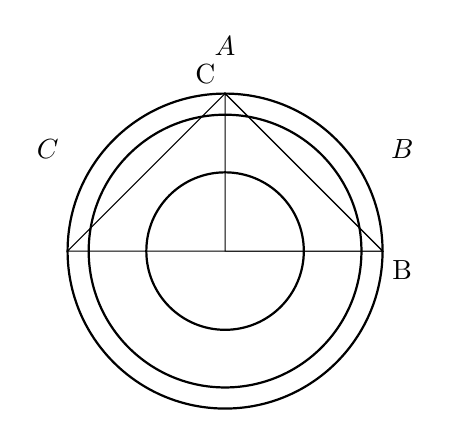
\begin{tikzpicture}[scale=2]
    % Draw the larger triangle
    \draw[fill=white] (-1,0) -- (1,0) -- (0,1) -- cycle;
    
    % Draw the smaller triangle
    \draw[fill=white] (0,0) -- (1,0) -- (0,1) -- cycle;
    
    % Label the vertices of the smaller triangle
    \node at (1,0) [below right] {B};
    \node at (0,1) [above left] {C};
    
    % Draw arcs to represent the angles
    \draw[thick] (0,0) circle (1);
    \draw[thick] (0,0) circle (0.866);
    \draw[thick] (0,0) circle (0.5);
    
    % Label the arcs
    \node at (90:1.3) {$A$};
    \node at (30:1.3) {$B$};
    \node at (150:1.3) {$C$};
\end{tikzpicture}
\end{document}